\documentclass[twocolumn,a4paper]{article}
\usepackage{graphicx}

\begin{document}
\title{The Exponential Function On A Single Page}
\author{Jens R. Larsen and Wikipedia}
\date{March 9 2022}
\maketitle

\section{Introduction}
The '''exponential function''' is a mathematical function denoted by $f(x)=\exp(x)$ or $e^x$ (where the argument $x$ is written as an exponent). The exponential function originated from the notion of exponentiation (repeated multiplication), and its persistent occurrence in pure and applied mathematics led mathematician Walter Rudin to denote the exponential function as "the most important function in mathematics". The value of the exponential function of 1 is called Euler's number: $\exp(1)\approx2.718$ and is a mathematical constant.

\section{The Exponential Function Numerically}
This short work has computed the exponential function numerically using a "quick-and-dirty" implementation. It involves treating the exponential function as a power series, represented as displayed in equation \ref{ExpDef}.
\begin{equation} \label{ExpDef}
	exp(x)  = \sum_{k = 0}^{\infty} \frac{x^k}{k!} = 1 + x + \frac{x^2}{2} + \frac{x^3}{6} + \frac{x^4}{24} +	\cdots
\end{equation}
Within the $C\#$ implementation the leading 10 orders have been included, while any higher orders have been assumed to be negligible. There are two special cases:
\begin{enumerate}
	\item If $x<0$ the function treats the negative value by being called recursively as $\left(\exp(-x)\right)^{-1}$
	\item If $x>1.8$, that is $x$ is larger than a specified precision, the function is called recursively as  
$\left(\exp(x/2)\right)^{2}$ in order to ensure that the required precision is obtained.
\end{enumerate}
\begin{figure}[h] \label{ExpPlot}
	%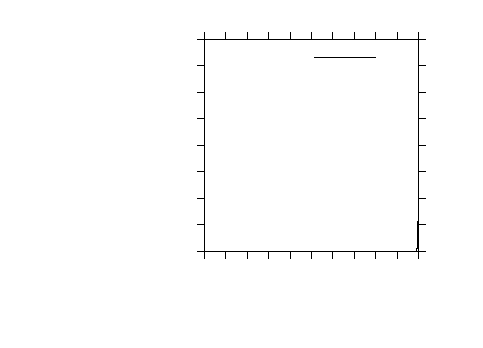
\includegraphics{exp_gnuplot}
	% GNUPLOT: LaTeX picture with Postscript
\begingroup
  \makeatletter
  \providecommand\color[2][]{%
    \GenericError{(gnuplot) \space\space\space\@spaces}{%
      Package color not loaded in conjunction with
      terminal option `colourtext'%
    }{See the gnuplot documentation for explanation.%
    }{Either use 'blacktext' in gnuplot or load the package
      color.sty in LaTeX.}%
    \renewcommand\color[2][]{}%
  }%
  \providecommand\includegraphics[2][]{%
    \GenericError{(gnuplot) \space\space\space\@spaces}{%
      Package graphicx or graphics not loaded%
    }{See the gnuplot documentation for explanation.%
    }{The gnuplot epslatex terminal needs graphicx.sty or graphics.sty.}%
    \renewcommand\includegraphics[2][]{}%
  }%
  \providecommand\rotatebox[2]{#2}%
  \@ifundefined{ifGPcolor}{%
    \newif\ifGPcolor
    \GPcolorfalse
  }{}%
  \@ifundefined{ifGPblacktext}{%
    \newif\ifGPblacktext
    \GPblacktexttrue
  }{}%
  % define a \g@addto@macro without @ in the name:
  \let\gplgaddtomacro\g@addto@macro
  % define empty templates for all commands taking text:
  \gdef\gplbacktext{}%
  \gdef\gplfronttext{}%
  \makeatother
  \ifGPblacktext
    % no textcolor at all
    \def\colorrgb#1{}%
    \def\colorgray#1{}%
  \else
    % gray or color?
    \ifGPcolor
      \def\colorrgb#1{\color[rgb]{#1}}%
      \def\colorgray#1{\color[gray]{#1}}%
      \expandafter\def\csname LTw\endcsname{\color{white}}%
      \expandafter\def\csname LTb\endcsname{\color{black}}%
      \expandafter\def\csname LTa\endcsname{\color{black}}%
      \expandafter\def\csname LT0\endcsname{\color[rgb]{1,0,0}}%
      \expandafter\def\csname LT1\endcsname{\color[rgb]{0,1,0}}%
      \expandafter\def\csname LT2\endcsname{\color[rgb]{0,0,1}}%
      \expandafter\def\csname LT3\endcsname{\color[rgb]{1,0,1}}%
      \expandafter\def\csname LT4\endcsname{\color[rgb]{0,1,1}}%
      \expandafter\def\csname LT5\endcsname{\color[rgb]{1,1,0}}%
      \expandafter\def\csname LT6\endcsname{\color[rgb]{0,0,0}}%
      \expandafter\def\csname LT7\endcsname{\color[rgb]{1,0.3,0}}%
      \expandafter\def\csname LT8\endcsname{\color[rgb]{0.5,0.5,0.5}}%
    \else
      % gray
      \def\colorrgb#1{\color{black}}%
      \def\colorgray#1{\color[gray]{#1}}%
      \expandafter\def\csname LTw\endcsname{\color{white}}%
      \expandafter\def\csname LTb\endcsname{\color{black}}%
      \expandafter\def\csname LTa\endcsname{\color{black}}%
      \expandafter\def\csname LT0\endcsname{\color{black}}%
      \expandafter\def\csname LT1\endcsname{\color{black}}%
      \expandafter\def\csname LT2\endcsname{\color{black}}%
      \expandafter\def\csname LT3\endcsname{\color{black}}%
      \expandafter\def\csname LT4\endcsname{\color{black}}%
      \expandafter\def\csname LT5\endcsname{\color{black}}%
      \expandafter\def\csname LT6\endcsname{\color{black}}%
      \expandafter\def\csname LT7\endcsname{\color{black}}%
      \expandafter\def\csname LT8\endcsname{\color{black}}%
    \fi
  \fi
    \setlength{\unitlength}{0.0500bp}%
    \ifx\gptboxheight\undefined%
      \newlength{\gptboxheight}%
      \newlength{\gptboxwidth}%
      \newsavebox{\gptboxtext}%
    \fi%
    \setlength{\fboxrule}{0.5pt}%
    \setlength{\fboxsep}{1pt}%
    %\definecolor{tbcol}{rgb}{1,1,1}%
\begin{picture}(4320.00,3024.00)%
    \gplgaddtomacro\gplbacktext{%
      \csname LTb\endcsname%%
      \put(682,767){\makebox(0,0)[r]{\strut{}$0$}}%
      \put(682,980){\makebox(0,0)[r]{\strut{}$2$}}%
      \put(682,1193){\makebox(0,0)[r]{\strut{}$4$}}%
      \put(682,1405){\makebox(0,0)[r]{\strut{}$6$}}%
      \put(682,1618){\makebox(0,0)[r]{\strut{}$8$}}%
      \put(682,1831){\makebox(0,0)[r]{\strut{}$10$}}%
      \put(682,2044){\makebox(0,0)[r]{\strut{}$12$}}%
      \put(682,2257){\makebox(0,0)[r]{\strut{}$14$}}%
      \put(877,484){\makebox(0,0){\strut{}$-3$}}%
      \put(1374,484){\makebox(0,0){\strut{}$-2$}}%
      \put(1871,484){\makebox(0,0){\strut{}$-1$}}%
      \put(2369,484){\makebox(0,0){\strut{}$0$}}%
      \put(2866,484){\makebox(0,0){\strut{}$1$}}%
      \put(3363,484){\makebox(0,0){\strut{}$2$}}%
      \put(3860,484){\makebox(0,0){\strut{}$3$}}%
    }%
    \gplgaddtomacro\gplfronttext{%
      \csname LTb\endcsname%%
      \put(209,1565){\rotatebox{-270}{\makebox(0,0){\strut{}$y$}}}%
      \put(2368,154){\makebox(0,0){\strut{}$x$}}%
      \put(2857,2190){\makebox(0,0)[r]{\strut{}$\mathrm{exp}(x)$}}%
      \put(2857,1970){\makebox(0,0)[r]{\strut{}$Tabular Values$}}%
      \put(2368,2693){\makebox(0,0){\strut{}Exponential Function}}%
    }%
    \gplbacktext
    \put(0,0){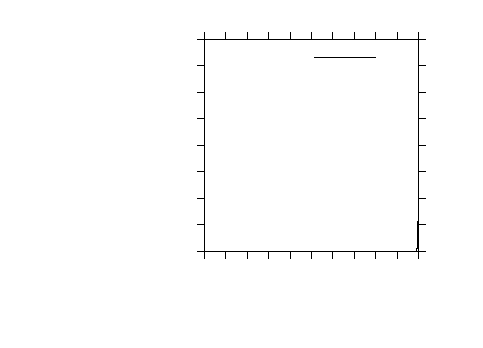
\includegraphics[width={216.00bp},height={151.20bp}]{exp_gnuplot}}%
    \gplfronttext
  \end{picture}%
\endgroup

\end{figure}
\section{Confirmation of Implementation}
With the aim of evaluating the implementation the exponential function has been plotted in figure \ref{ExpPlot} against table values. In order to validate of the exponential function implementation as a power series it has been plotted against tabular values for the interval $[-3<x\leq3]$. The correlation found is acceptable and this work thus concludes that the implementation yields a reasonable treatment of the exponential function.



\end{document}
